\section{Analyse der Pakete bei WebWhatsApp}\label{sec:kaptiel}
\subsection{Ziel}
Ziel dieses Versuches ist es, zu ermitteln wie die Anmeldung, der Aufbau einer Session 
und der Nachrichtenverkehr bei WebWhatsApp funktioniert. Welche Protokolle werden
verwendet? Welche Pakete werden in welcher Reihenfolge versendet und empfangen?\\
\textbf{Aktionen:}
\begin{enumerate}
    \item Der Laptop meldet sich über einen Browser bei WebWhatsApp an. Er ist bereits über das Smartphone registriert.
    \item Nach der erfolgreichen Anmeldung, werden zwei Nachrichten versendet.
\end{enumerate}

\subsection{Aufbau}
\begin{center}
    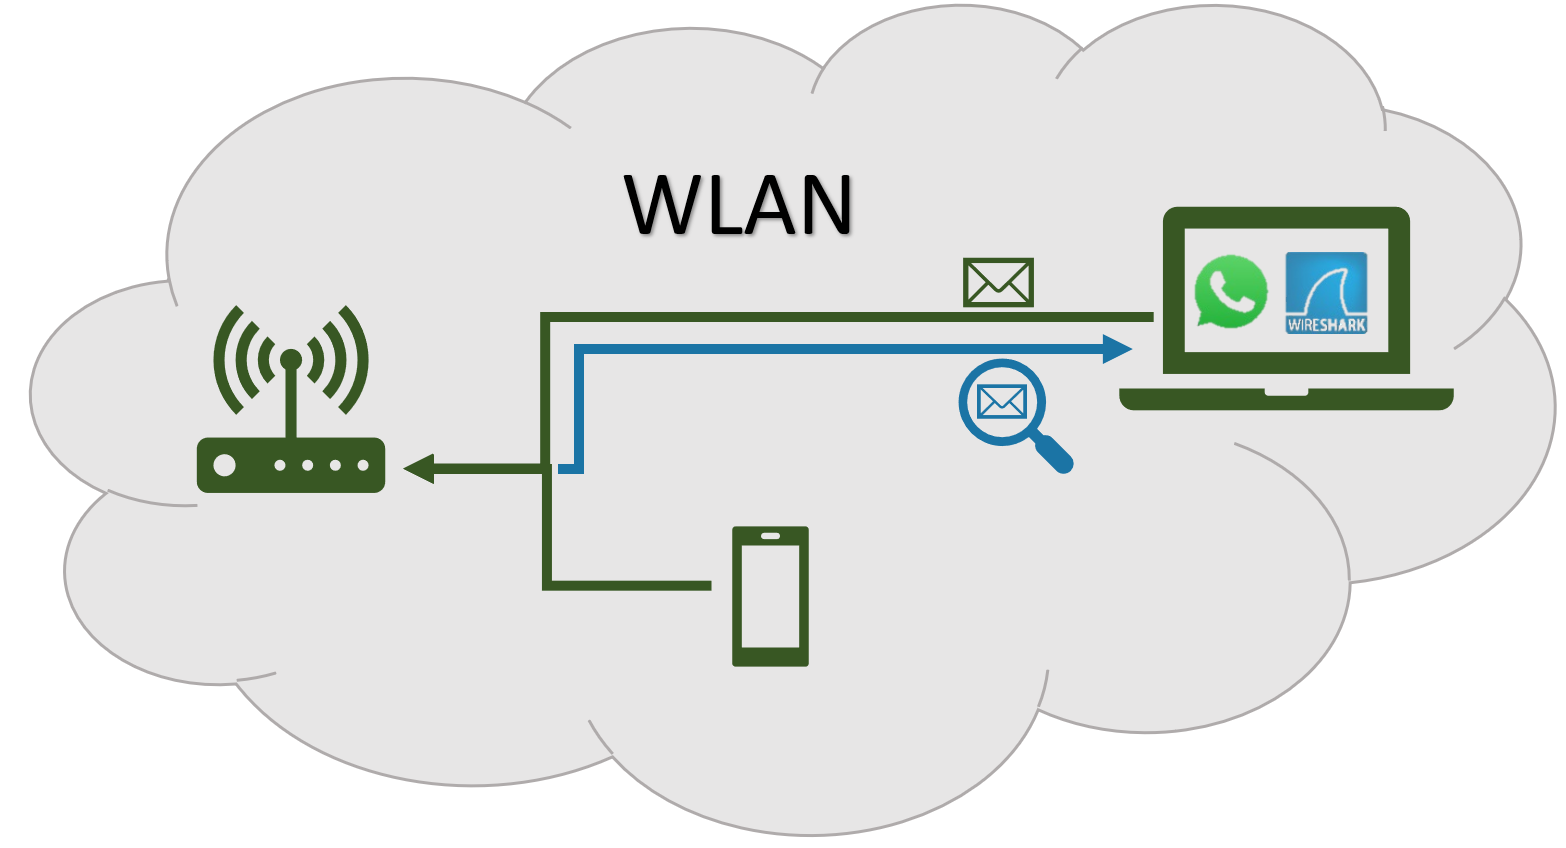
\includegraphics[width=9cm]{Aufbau}
\end{center}

\begin{description}
    \item \textbf{Laptop}
        \begin{description}
            \item \textit{WebWhatsApp}: 
                Über diesen Laptop wird WebWhatsApp aufgerufen. Der Client ist 
                bereits auf registriert. 
            \item \textit{Wireshark}:
                Zusätzlich ist Wireshark installiert um die gesamte Netzwerkkommunikation
                zu analysieren.
        \end{description}
    \item \textbf{Smartphone}
    \begin{description}
       \item Das Smartphone über das der Laptop Client bei WhatsApp registriert ist, muss
            sich im Internet befinden. In diesem Fall ist es im gleichen WLAN (müsste es aber nicht sein). 
    \end{description}
\end{description}

\subsection{Analyse mit Wireshark}
\subsubsection{Vorgehen und erster Überblick}
Da zunächst noch nicht bekannt ist, welche Pakete von WhatsApp verschickt werden.
Wird das Capturing von Wireshark ohne Capture Filter ausgeführt. Nachteil ist, 
dass dadurch viel zu viele Pakete angezeigt werden z.B. verschiedene Dropbox Jobs. 
Deshalb müssen zunächst die für die WhatsApp-Analyse relevanten Pakete bzw. Streams
gefunden werden. 
Die einfachste Möglichkeit ist es nach der IP-Adresse zu filtern. 
WebWhatsApp verwendet IPv6 und hat die Adresse: \texttt{2a03:2880:f22d:c5:face:b99c:0:167}. 
Mit diesem Display-Filter ist es möglich das 'Client Hello' Paket vom TLS.v3-Handshake zu finden. 

\begin{center}
    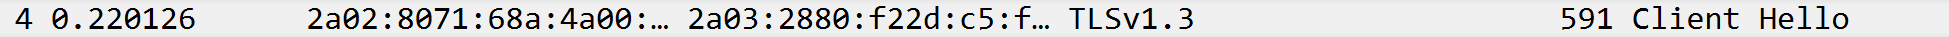
\includegraphics[width=14cm]{ClientHelloTLS}
\end{center}
Dieser SSL-Session kann im Anschluss gefolgt werden. So wird der gesamte SSL-Stream angezeigt.

\begin{center}
    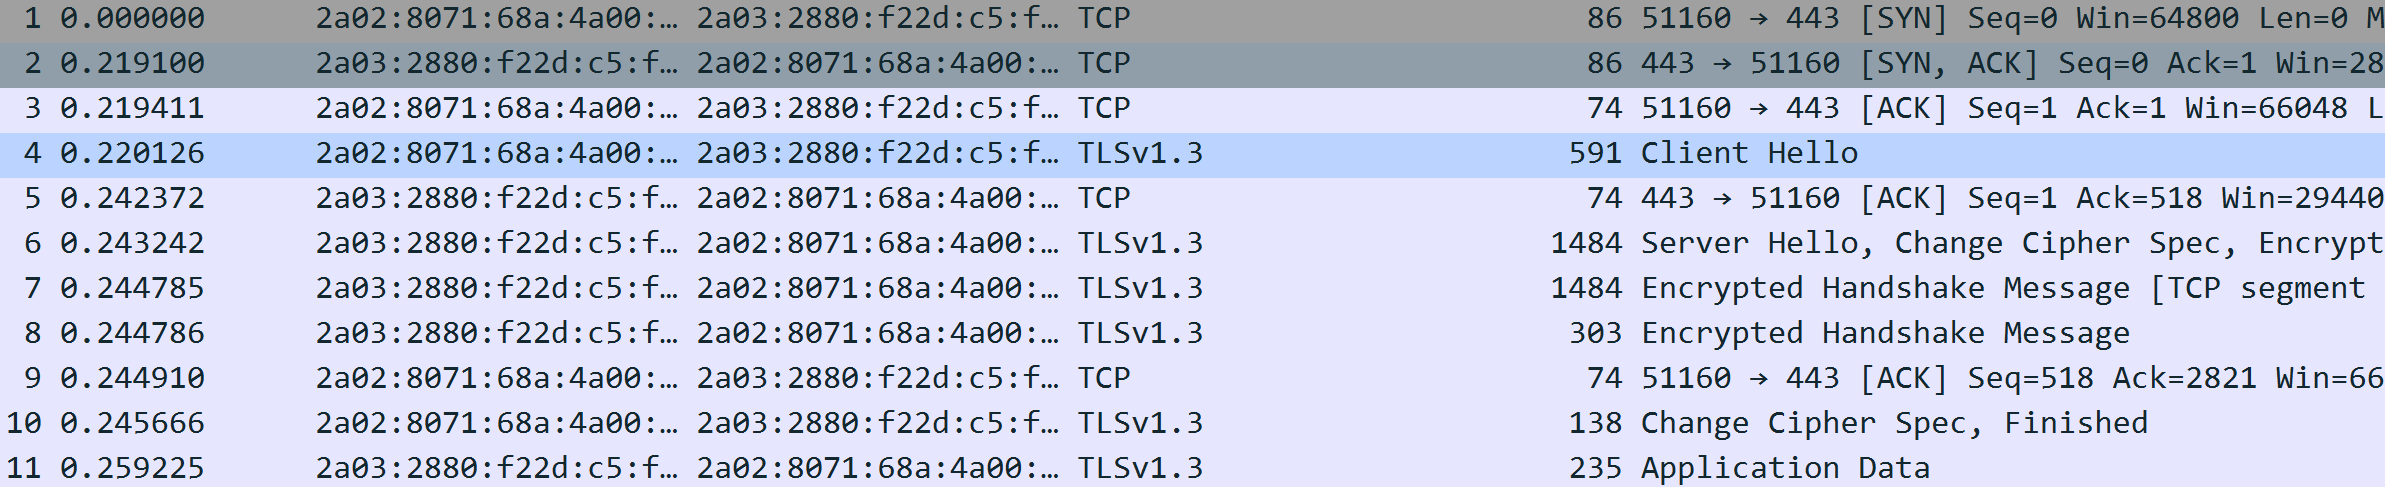
\includegraphics[width=15cm]{WhatsAppFilteredOverview}
\end{center}

In diesem Wireshark-Ausschnitt sind 4 Aktionen sichtbar:
\begin{enumerate}
    \item TCP Handshake
    \item TLSv1.3 Handshake
    \item TLS Cipher-Suite Einigung
    \item Übertragung der Daten von WhatsApp    
\end{enumerate}

Diese einzelnen Aktionen, die notwendig zum Aufbau der Session sind, 
werden im Folgenden genauer analysiert.

\subsubsection{TCP Handshake}
Die ersten drei Pakete des Wireshark-Snippets stellen den TPC Handshake dar.

\begin{center}
    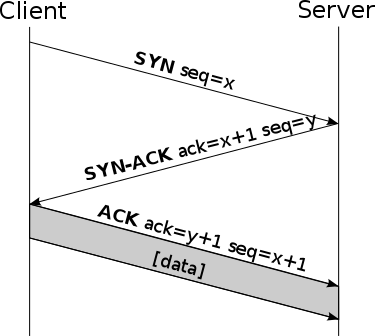
\includegraphics[width=4.5cm]{TCPHandshake0}
\end{center}
Dieser Handshake ist notwendig um eine Verbindung zwischen den beiden Sockets von Client
und Server herzustellen.

\begin{center}
    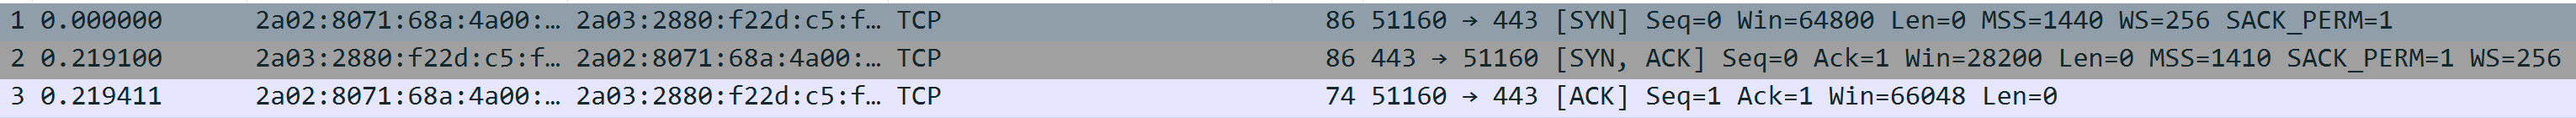
\includegraphics[width=15cm]{TLSHandshake1}
\end{center}
In diesem Wireshark-Snippet ist genau dieser Ablauf zu erkennen.
Wireshark bietet die Möglichkeit, die Pakete in einem Flowchart anzuzeigen. 
Dieser ist für einen Überblick sehr hilfreich.
\begin{center}
    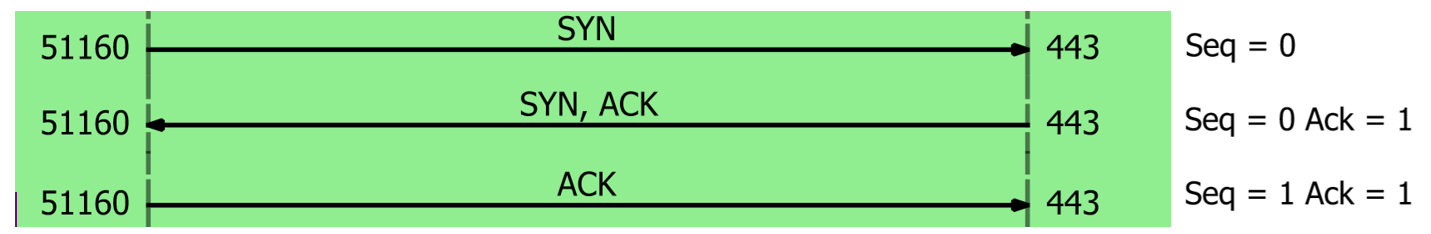
\includegraphics[width=10cm]{TCPHandshakeOverview} 
\end{center}

Zunächst sendet der Laptop (mit WebWhatsApp) das \texttt{SYN-Paket} mit einer Sequenznummer.

\begin{center}
    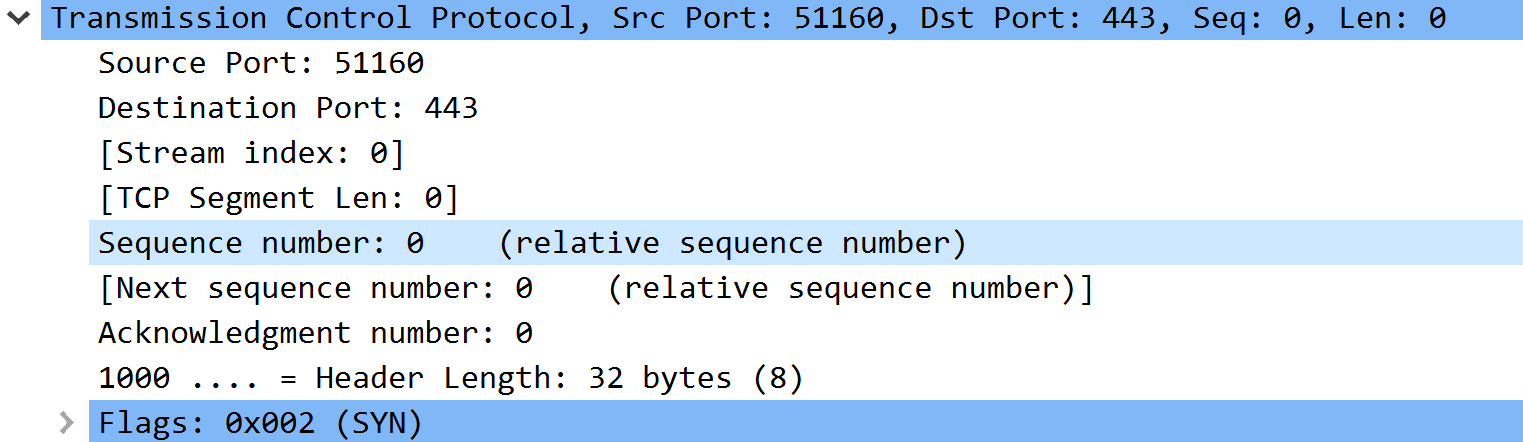
\includegraphics[width=10cm]{TCPHandshake1}
\end{center}

In diesem Fall ist die \texttt{Sequenznummer = 0}
Der Server antwortet mit einem \texttt{SYN-ACK-Paket}.

\begin{center}
    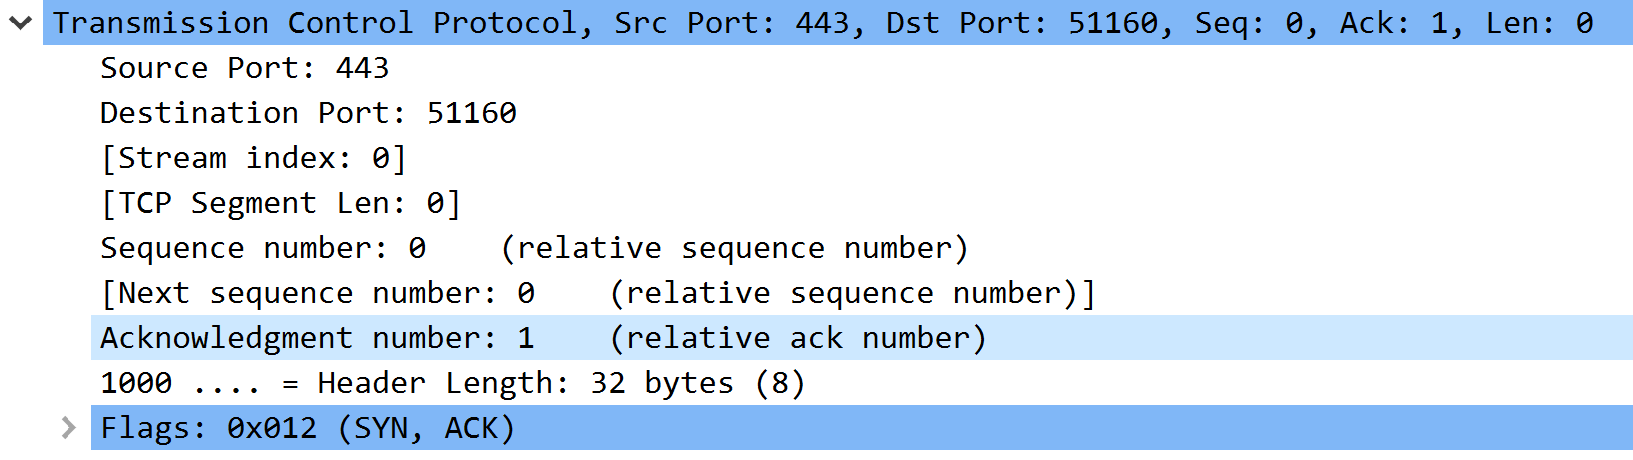
\includegraphics[width=10cm]{TCPHandshake2}
\end{center}

Dort ist die \texttt{Acknowledgementnummer = 1} und eine neue \texttt{Sequenznummer = 0}. 
Zum Abschluss des Handshakes sendet der Client dem Server seinerseits ein \texttt{ACK-Packet}.

\begin{center}
    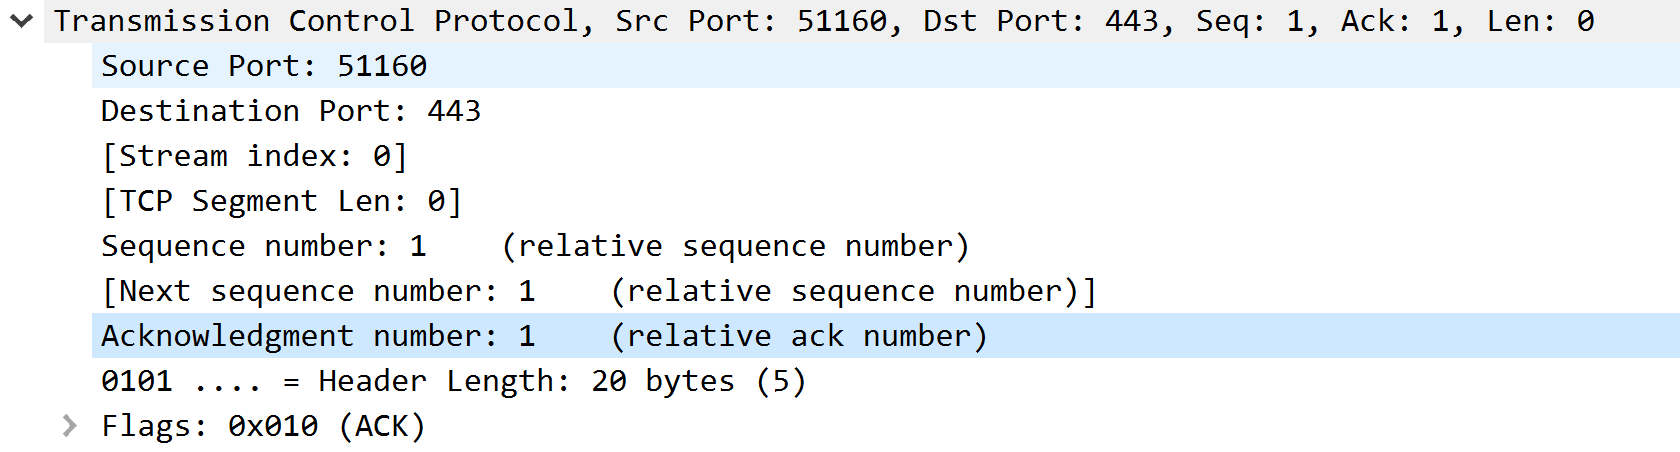
\includegraphics[width=10cm]{TCPHandshake3}
\end{center}

\subsubsection{TLSv1.3 Handshake}
Für den TLSv1.3 Handshake sieht der Flowchart der von Wireshark generiert
wird wie folgt aus.

\begin{center}
    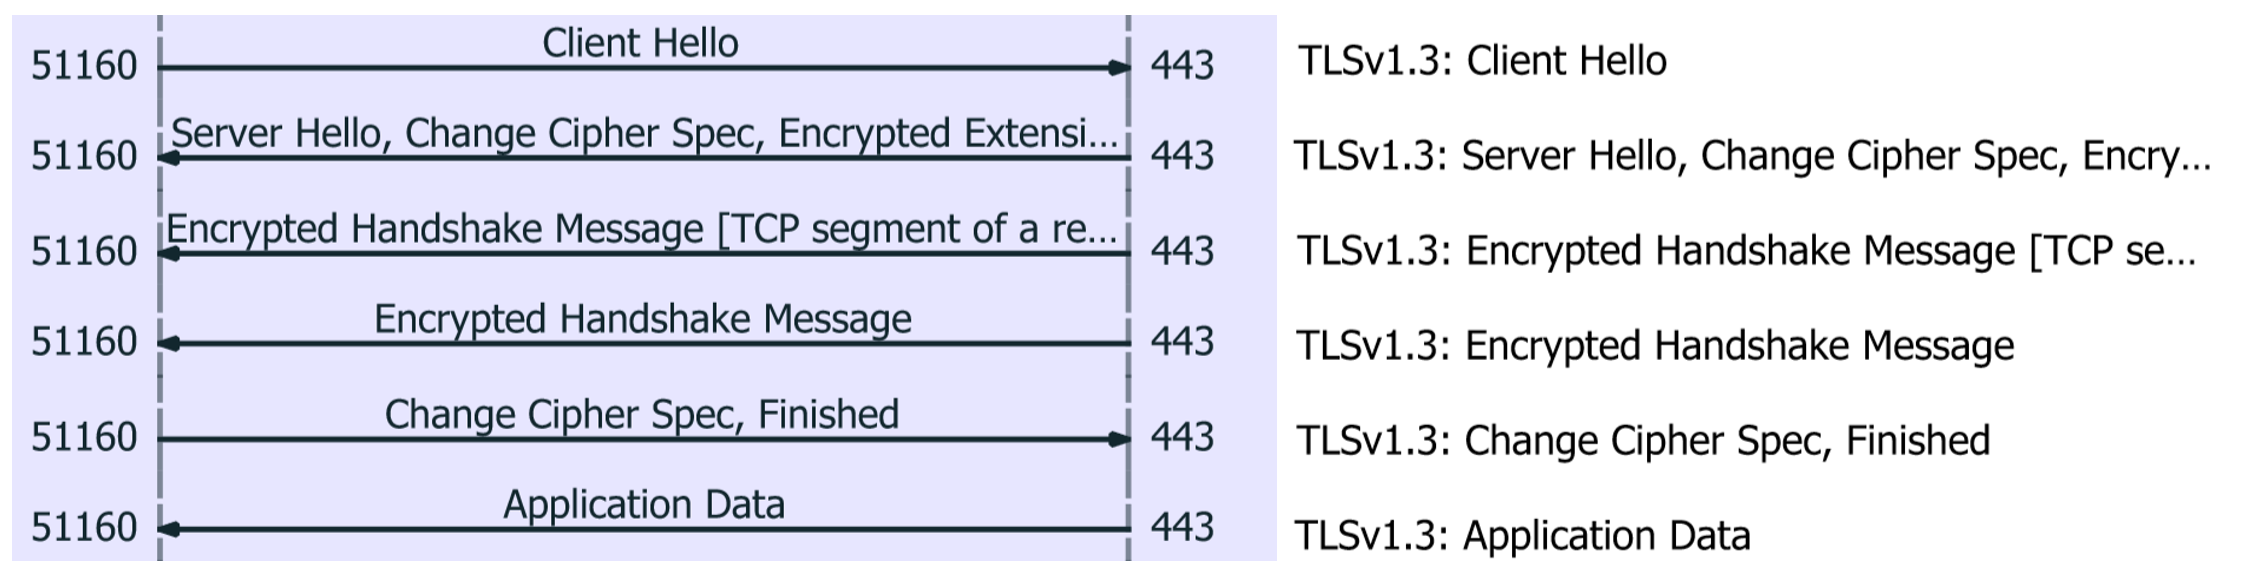
\includegraphics[width=15cm]{TLSHandshakeOverview}
\end{center}

\textbf{Client Hello}\\
In dem Paket ist nun die Secure Sockets Layer interessant.
\begin{center}
    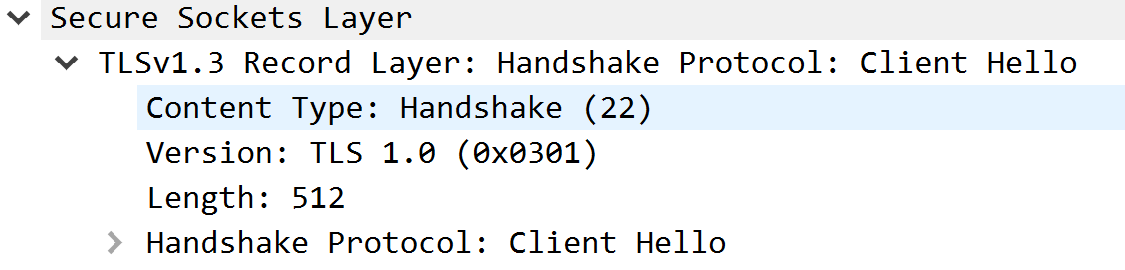
\includegraphics[width=10cm]{TLSHandshakeSSLClientHello}
\end{center}
Hier ist zu erkennen, dass die Version 1.3 von TLS verwendet wird. Dieses Paket ist nach
dem Handshake-Protokoll das \texttt{Client Hello}-Paket.
Schaut man sich das Handshake Protokoll genauer an, können weitere Details über
die Art der Verschlüsselten Kommunikation eingesehen werden.
\begin{center}
    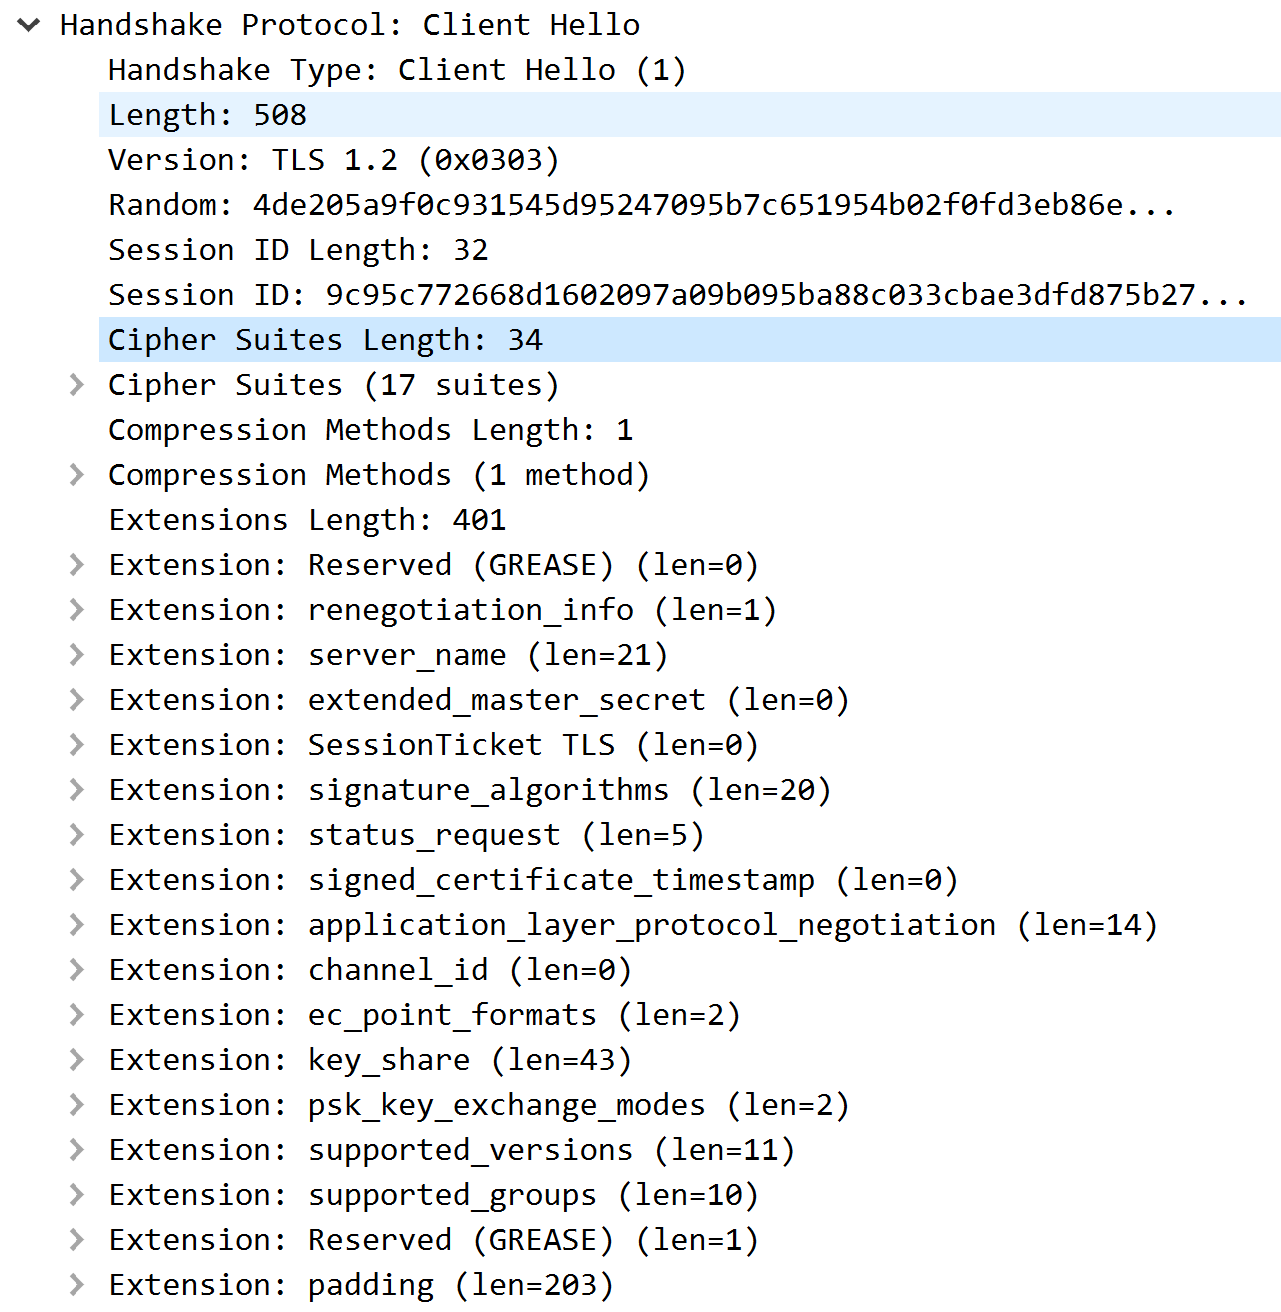
\includegraphics[width=10cm]{TLSHandshakeProtokollClientHello}
\end{center}
Es wird eine Liste der verfügbaren Chipher-Suites angegeben.Aus dieser Liste wird vom Server eine
Suite ausgewählt. Zusätzlich wird eine 32bit lange SessionID übergeben. 
Weitere Erweiterungen des TLSv1.3 Protokolls geben Einblick in (einige interessante Beispiele):
\begin{itemize}
    \item Signatur des Clients (mit Status und Timestamp)
    \item Öffentlichen Schlüssel des Clients
    \item Art der verwendeten Verschlüsselung
\end{itemize}
Die Art der Verschlüsselung gibt hier an, dass eine Deffie-Hellman-Verschlüsselung verwendet
werden soll.
\begin{center}
    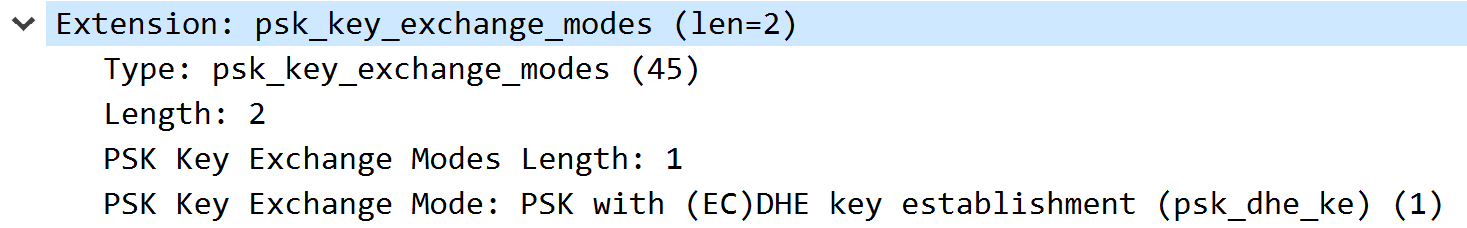
\includegraphics[width=10cm]{TLSHandshakePublicKeyProtocol}
\end{center}
Unter dem Punkt Exchange Mode wird angegeben\texttt{PSK with (EC)-DHE key establishment}.
Der Server verfügt nun also über den Public Secret Key (PSK) und weiß, dass ein 
Eliptic-Curve-Deffie-Hellman-Verfahren (EC-DHE) 
verwendet werden soll. \\

\textbf{Antwort vom Server auf das Client-Hello Paket: Server Hello}\\
Der Server versendet gleich 3 Pakete zurück an den Client. 
\begin{enumerate}
    \item \texttt{Server Hello, Change Cipher Suite, Encrypted Extensions}
    \item \texttt{Encrypted Handshake Message [TCP segment of a re....]}
    \item \texttt{Encrypted Handshake Message}
\end{enumerate}
Das erste Paket beinhaltet wiederum drei verschiedene SSL Frames.
\begin{enumerate}
    \item \texttt{Handshake Protocol: Server Hello}
    \item \texttt{Change Cipher Spec Protocol: Change Cipher Spec}
    \item \texttt{Handshake Protocol: Encrypted Extensions}
\end{enumerate}

Das Folgende Bild zeigt die Inhalte des ersten Pakets.

\begin{center}
    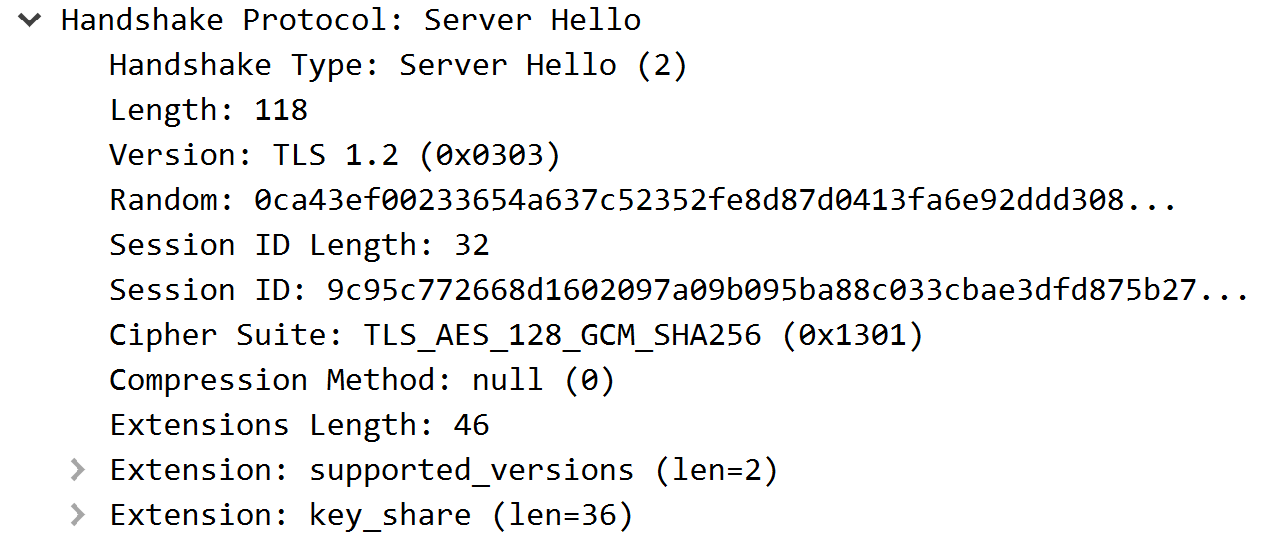
\includegraphics[width=10cm]{TLSHandshakeServerHello}
\end{center}

Im Server Hello Paket teilt der Server dem Client die gewählte Cipher-Suite mit.
WhatsApp verwendet für die SSL verschlüsselung das symmetrische Verfahren 
\texttt{AES128} im \texttt{GCM Modus}. Für den Hashwert wird das Verfahren \texttt{SHA256} gewählt. 
Außerdem wird auch die SessionID die der Client im \texttt{Client Hello Paket} mitgesendet hat erneut mitgesendet. 
Auch der Server sendet seinen öffentlichen Schlüssel zum Client. Sowohl Client als auch Server sind nun 
im Besitz der jeweiligen öffentlichen Schlüssel und können nun verschlüsselt miteinander 
Kommunizieren. Der zweite Frame zeigt ausschließlich, dass die Cipher-Suite geändert wurde. 
Der letzte Frame enthält wieder mehr Informationen. Hier wird die ALPN (Application Layer Protocol Negotation) festgelegt. 
ALPN wird dazu verwendet, auszuhandeln welches Protokoll innerhalb der TLS-Verbindung verwendet wird. 
\cite{ALPN}
Das nächste Paket ist das \texttt{Encrypted Handshake Message [TCP segment of a reassembled PDU]}
PDU steht hier für \texttt{Protocol Data Unit}. Wireshark erkennt hier, dass es sich bei dem Paket um 
ein Teil eines anderen Pakets für ein Protokoll überhalb von TCP handelt. \cite{WSHelp1}
Viel mehr letzt sich aus diesem und auch dem nächsten Paket nicht auslesen, da diese Pakete bereits verschlüsselt sind.


\textbf{Change Cipher Suite, Finished}\\
Das letzte Paket, dass zum Verbiungsaufbau vom Client an den Server gesendet wird ist das \texttt{Change Cipher Spec, Finished Paket}. 
Der Client teilt dem Server mit, dass die Änderung der Cipher-Suite erhalten hat. Außerdem teilt der Client mit, dass
auch von seiner Seite der TLS Handshake beendet ist.

\textbf{Application Data}\\
Die folgenden Pakete enhalten Applikations Daten. Diese sind, wie zuvor im Handshake ausgehandelt, mit einem AES Schlüssel verschlüsselt.
\begin{center}
    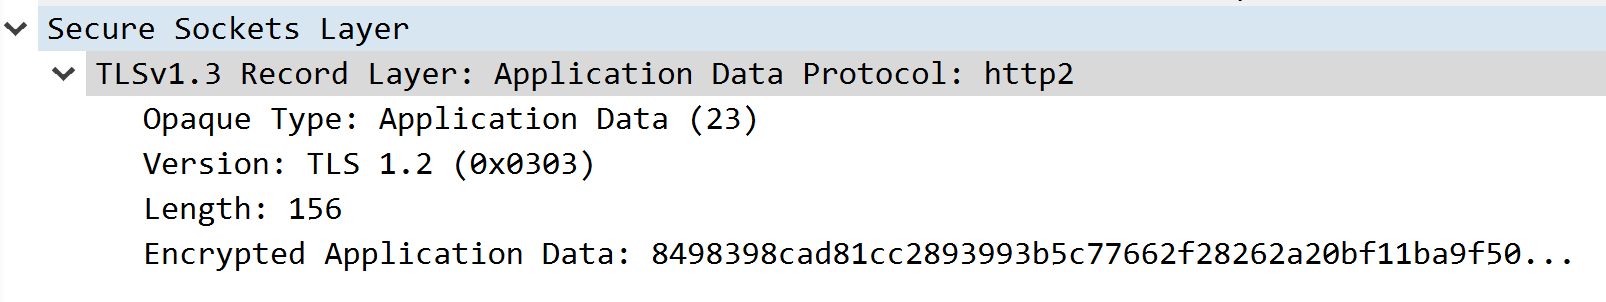
\includegraphics[width=15cm]{TLSApplicationData}
\end{center}